%
% The Quantum Sneakernet
%

\section{The quantum Sneakernet\texttrademark}\index{Sneakernet}\label{sec:sneakernet}

\sectionby{Simon Devitt}\index{Simon Devitt}

\comment{To do. Simon Devitt.}

\begin{figure}[!htbp]
\if 1\doublecol
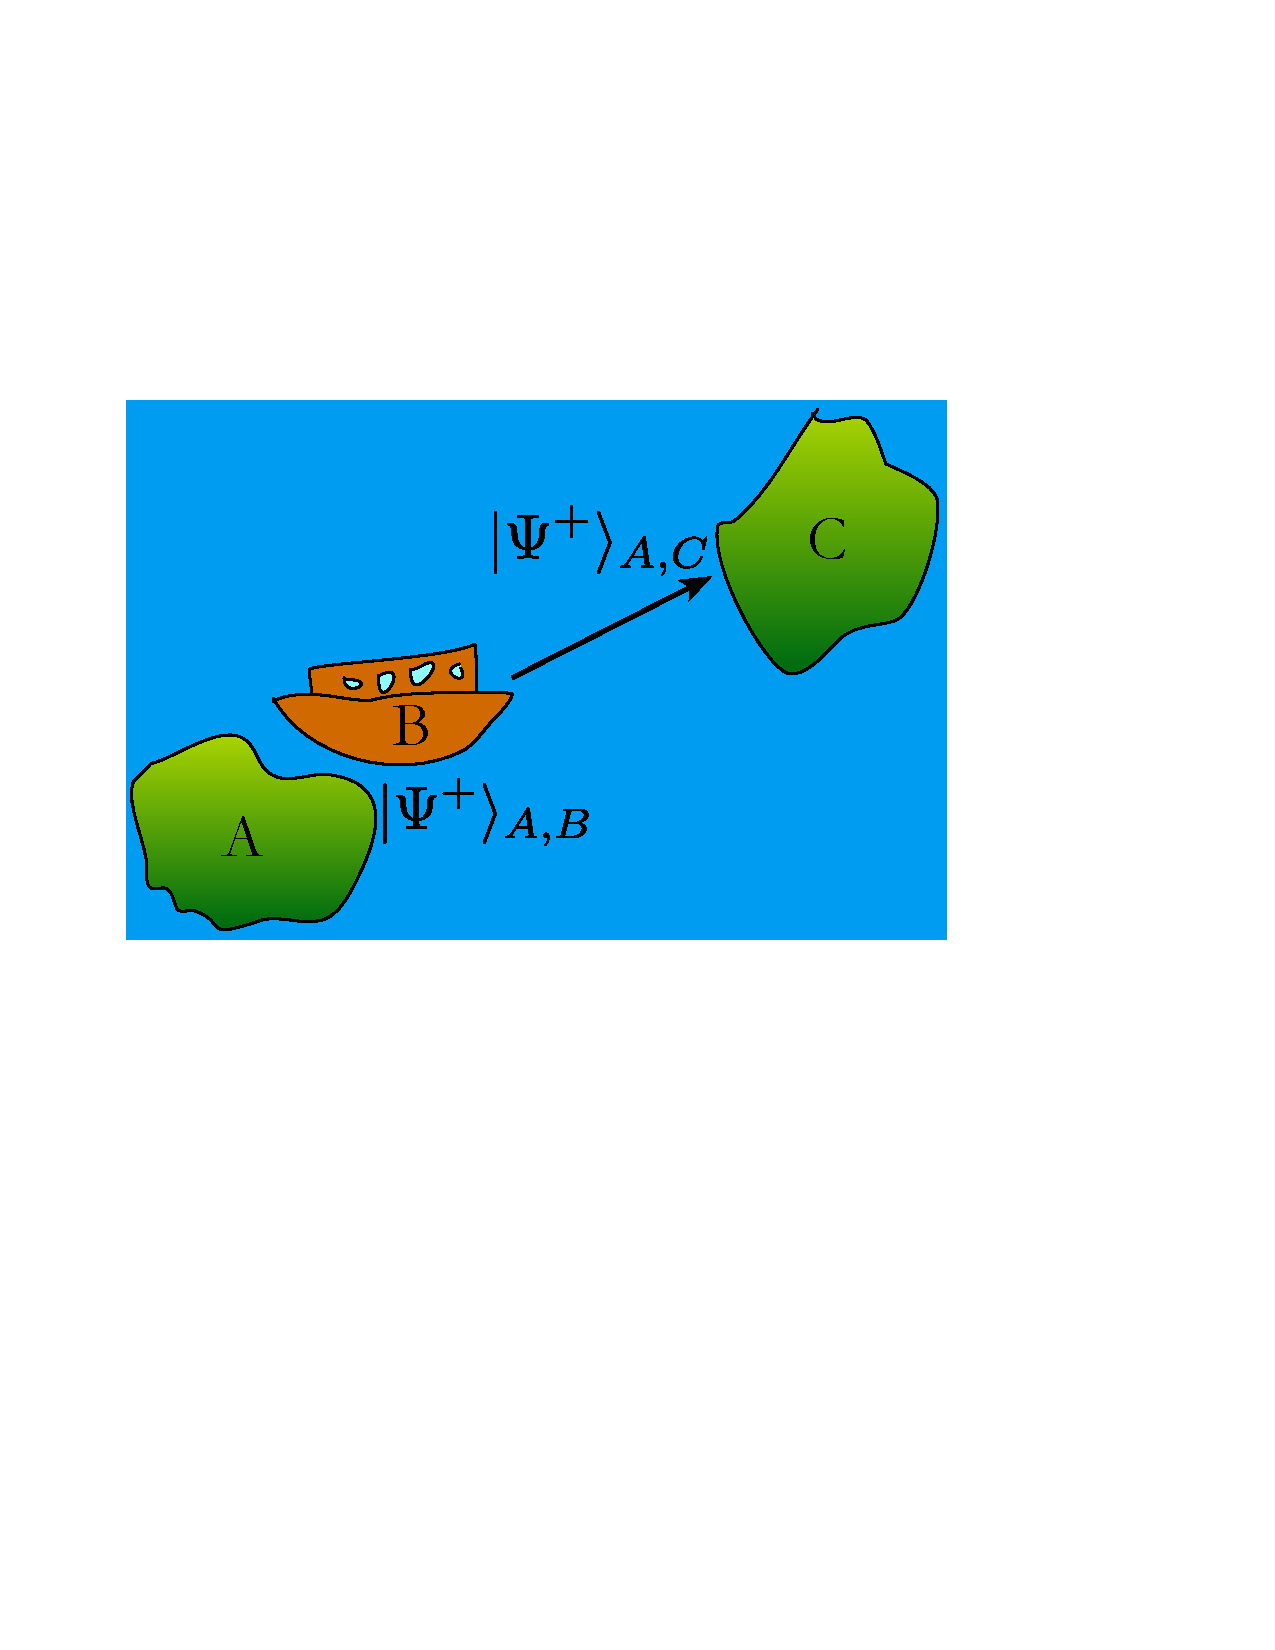
\includegraphics[clip=true, width=0.475\textwidth]{sneakernet_boat}
\else
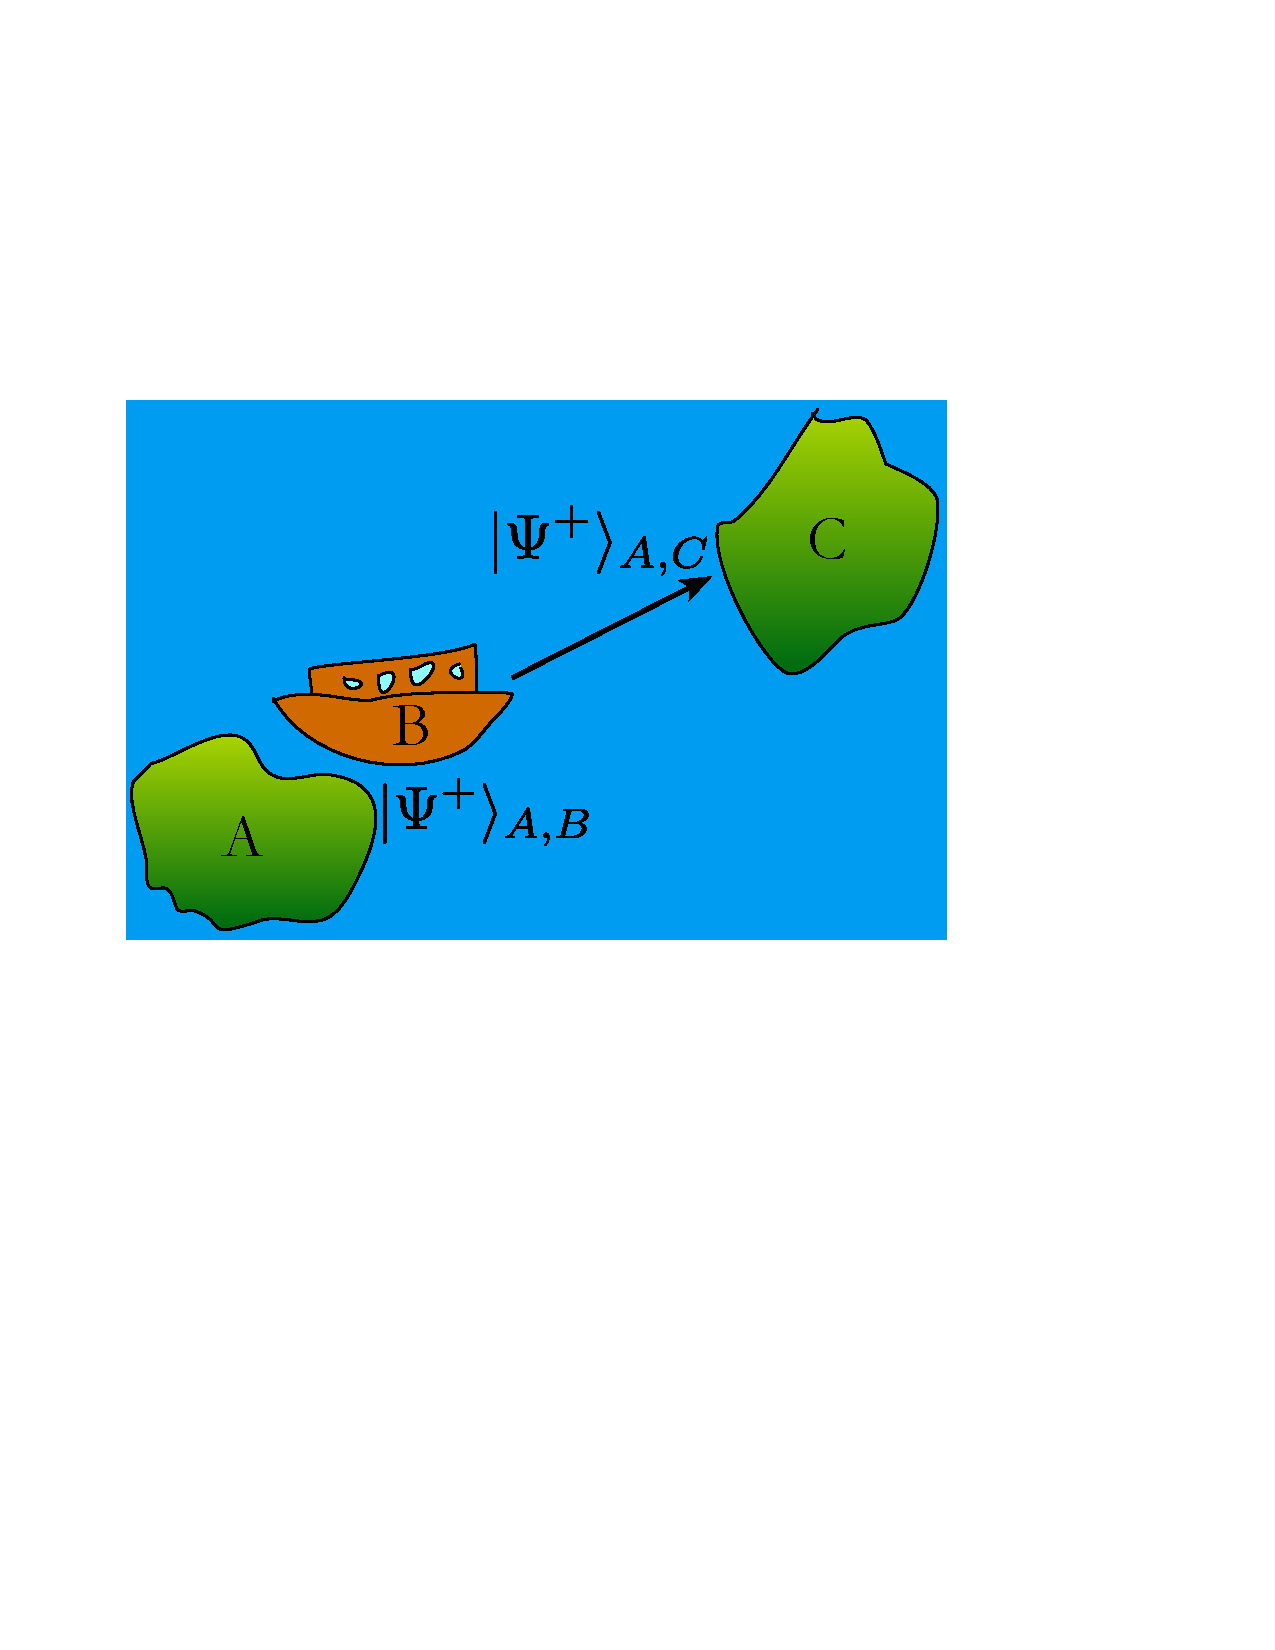
\includegraphics[clip=true, width=0.7\textwidth]{sneakernet_boat}
\fi
\captionspacefig \caption{In the quantum Sneakernet\texttrademark entanglement distribution protocol, rather than using conventional flying qubits, we take highly error-corrected stationary qubits and physically transport them over long distances as freight. The error correction must be sufficient to maintain coherence over the time-scale of the journey, which could be anything from hours (when flying) to weeks (by sea\footnote{Or indefinitely if the destination is Australia and you're fleeing war crimes.}). The mode of transport only transports one half of an error-corrected Bell pair, transferring the initial entanglement between source and vessel, $\ket{\Psi^+}_{A,B}$, to be between source and destination, $\ket{\Psi^+}_{A,C}$. Because all Bell pairs are identical and infinitely reproducible, latency presents no problem. For example, when using a Bell pair to teleport a qubit over long distances, when the Bell pair arrives is unimportant, as long as it's available at the time of teleportation. Thus, our Bell pair cargo carriers can simply operate in the background, transporting Bell pairs with as much bandwidth as possible, which may then be buffered by the recipient until required, latency being unimportant provided the coherence lifetime of the error correcting code is long enough.}\label{fig:sneakernet_boat}	
\end{figure}
